\documentclass[11pt,a4paper]{article}
\usepackage[utf8]{inputenc}
\usepackage[T1]{fontenc}
\usepackage{tgpagella}
\usepackage[spanish]{babel}
\usepackage{geometry}
\usepackage{booktabs}
\usepackage{xcolor}
\usepackage{titlesec}
\usepackage{fancyhdr}
\usepackage[parfill]{parskip}
\usepackage[expansion=false]{microtype}
\usepackage{hyperref}
\usepackage{setspace}
\usepackage{graphicx}
\usepackage{needspace}

\widowpenalty=10000
\clubpenalty=10000
\displaywidowpenalty=10000

\geometry{top=3.0cm,bottom=3.0cm,left=3.5cm,right=3.5cm}
\setlength{\parskip}{0.65em}
\setlength{\parindent}{0em}

\definecolor{azulai}{RGB}{30,80,140}
\definecolor{doradoai}{RGB}{140,90,0}
\definecolor{grisai}{RGB}{70,70,70}

\titleformat{\section}{\Large\bfseries\color{azulai}}{}{0em}{}[{\color{azulai}\titlerule[0.5pt]}]
\titlespacing*{\section}{0pt}{1.4em}{0.5em}

\titleformat{\subsection}{\large\bfseries\color{doradoai}}{}{0em}{}
\titlespacing*{\subsection}{0pt}{1.0em}{0.35em}

\titleformat{\subsubsection}{\normalsize\bfseries\color{grisai}}{}{0em}{}
\titlespacing*{\subsubsection}{0pt}{0.7em}{0.25em}

\pagestyle{fancy}\fancyhf{}
\rhead{\textcolor{grisai}{\small Maite Barragan — Arquitectura Interna}}
\lhead{\textcolor{grisai}{\small Plutón · Casa 8 · Casa 12 · Quirón · Lilith}}
\cfoot{\textcolor{grisai}{\small\thepage}}
\renewcommand{\headrulewidth}{0.3pt}

\hypersetup{colorlinks=true,linkcolor=azulai,urlcolor=azulai}
\setstretch{1.25}
\tolerance=1500
\emergencystretch=4em

\begin{document}

\begin{titlepage}
  \centering
  \vspace*{1.5cm}
  {\Huge\bfseries\color{azulai} Plutón · Casa 8 · Casa 12}\\[0.35cm]
  {\Huge\bfseries\color{azulai} Quirón · Lilith}\\[0.5cm]
  {\large\color{grisai} Arquitectura Interna}\\[0.3cm]
  {\small\itshape\color{grisai} Sombra, herida, intimidad y profundidad psíquica}\\[2cm]
  {\huge\color{doradoai} Maite Barragan}\\[1.5cm]
  {\Large 07/01/1971 \quad 12:15}\\[0.3cm]
  {\Large Pamplona, España}\\[0.3cm]
  {\normalsize Lat: 42.8157° \quad Lon: -1.6522° \quad UTC+01:00}\\[0.3cm]
  {\normalsize Ascendente: Aries 6°18' \quad
    MC: Capricornio 3°11'}\\[2cm]

  \begin{tabular}{ll}
    \textbf{Plutón:}  & Virgo — Casa 6 29°42' (retrógrado) \\
    \textbf{Quirón:}  & Aries — Casa 12 6°04' \\
    \textbf{Lilith:}  & Virgo — Casa 6 13°58' \\
    \textbf{Casa 8:}  & Escorpio \\
    \textbf{Casa 12:} & Acuario \\
  \end{tabular}\\[2cm]

  \vfill
  {\small Generado el 20/05/2026}
\end{titlepage}

\tableofcontents
\newpage

\section{Datos de referencia}

\begin{center}
\begin{tabular}{llll}
  \toprule
  \textbf{Punto} & \textbf{Signo} & \textbf{Casa} & \textbf{Posición} \\
  \midrule
  Plutón (retrógrado) & Virgo & 6 & 29°42' \\
  Quirón & Aries & 12 & 6°04' \\
  Lilith          & Virgo & 6 & 13°58' \\
  Casa 8          & Escorpio             & ---                  & --- \\
  Casa 12         & Acuario            & ---                  & --- \\
  Ascendente      & Aries         & ---                  & 6°18' \\
  Medio Cielo     & Capricornio          & ---                  & 3°11' \\
  \bottomrule
\end{tabular}
\end{center}

\vspace{0.5cm}
\textbf{Aspectos relevantes:}

\begin{center}
\begin{tabular}{lllll}
  \toprule
  \textbf{Punto 1} & \textbf{Asp.} & \textbf{Punto 2} & \textbf{Aspecto} & \textbf{Orbe} \\
  \midrule
  Plutón & sex & Venus & Sextil & 0.7° \\
  Plutón & sex & Júpiter & Sextil & 0.9° \\
  Plutón & cua & Mercurio & Cuadratura & 1.9° \\
  Plutón & tri & Luna & Trígono & 1.9° \\
  Plutón & sex & Neptuno & Sextil & 2.5° \\
  Plutón & opo & Quirón & Oposición & 6.4° \\
  Quirón & tri & Neptuno & Trígono & 3.9° \\
  Lilith & tri & Saturno & Trígono & 1.8° \\
  Lilith & tri & Sol & Trígono & 2.5° \\
  \bottomrule
\end{tabular}
\end{center}

\begin{center}
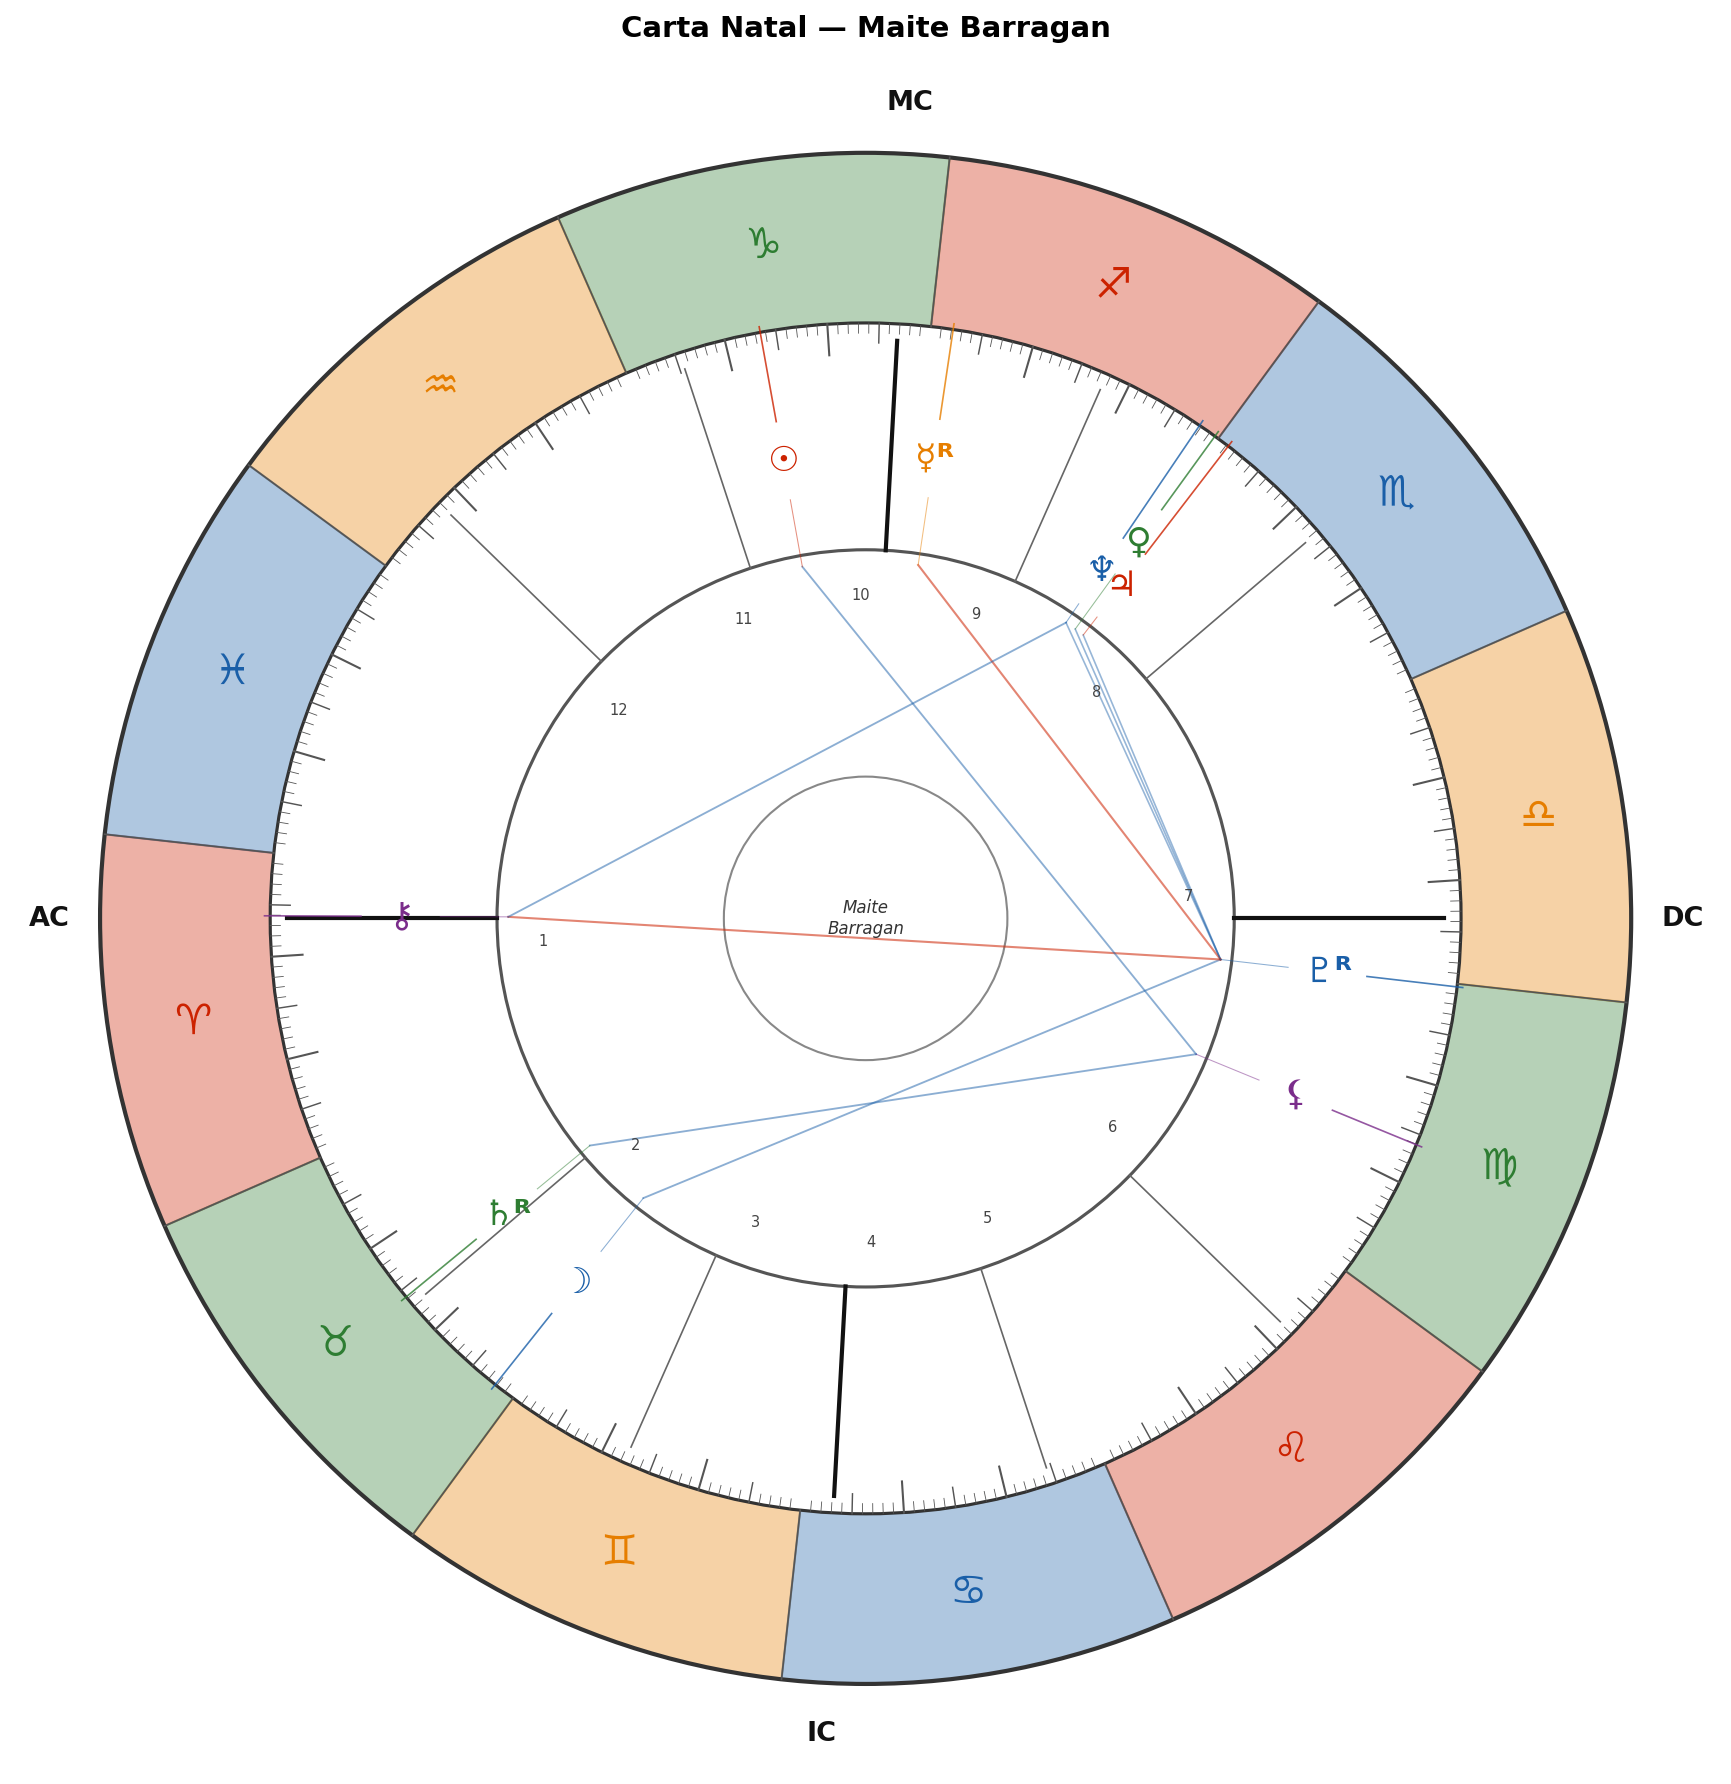
\includegraphics[width=0.72\textwidth]{Maite_Barragan_rueda.png}
\end{center}

\Needspace{3\baselineskip}

\section{Interpretación}

\begin{center}
{\small\itshape
Este documento no busca definirte. Se acerca a zonas donde pueden aparecer intensidad,\\
defensa, herida, vulnerabilidad, deseo, retiro o dificultad para poner en palabras lo que ocurre.
}
\end{center}

\vspace{0.8cm}

\Needspace{10\baselineskip}
\vspace{0.4cm}

\subsection{1. Marco general}

Este documento entra en zonas de la carta que suelen vivirse con más intensidad, más defensa o más dificultad para nombrar. No describe una identidad fija ni una condena personal. Se acerca a lugares donde pueden aparecer miedo, control, vergüenza, deseo, aislamiento, dependencia, heridas antiguas o reacciones difíciles de comprender desde fuera.

Plutón en Virgo, Casa 6: muestra dónde puedes vivir procesos intensos de transformación, pérdida de control, apego, defensa o profundidad emocional.
Quirón en Aries, Casa 12: muestra una zona especialmente sensible, donde puede haber herida, inseguridad, vergüenza o necesidad de protección.
Lilith en Virgo, Casa 6: muestra una parte de ti menos domesticable, más instintiva, que puede reaccionar con fuerza cuando se siente atrapada, reducida o invadida.

La Casa 8 en Escorpio habla de cómo atraviesas la vulnerabilidad, la intimidad, la pérdida, la confianza y los vínculos que remueven profundamente.
La Casa 12 en Acuario habla de cómo vives el retiro, la sensibilidad, el agotamiento emocional, lo inconsciente y aquello que cuesta poner en palabras.

Aspectos principales observados en este bloque: Plutón–Venus en sextil (orbe 0.69°), Plutón–Júpiter en sextil (orbe 0.91°), Plutón–Mercurio en cuadratura (orbe 1.85°), Plutón–Luna en trígono (orbe 1.86°), Plutón–Neptuno en sextil (orbe 2.49°), Plutón–Quirón en oposición (orbe 6.36°), Quirón–Neptuno en trígono (orbe 3.87°), Lilith–Saturno en trígono (orbe 1.83°), Lilith–Sol en trígono (orbe 2.54°).

\Needspace{10\baselineskip}
\vspace{0.4cm}

\subsection{2. Plutón — Intensidad, control y transformación}

\Needspace{6\baselineskip}
\subsubsection*{Plutón en Virgo — Casa 6 (retrógrado)}

Plutón en Virgo muestra una intensidad profunda ligada al control, la mejora, el cuerpo, el trabajo y la necesidad de hacerlo bien. Puede haber una exigencia interna fuerte, como si cualquier error pudiera abrir una grieta difícil de sostener.

La sombra puede aparecer como perfeccionismo, culpa, autoobservación dura o dificultad para descansar si algo no está resuelto. A veces puedes intentar ordenar por fuera una angustia que en realidad pide ser escuchada por dentro.

La transformación pasa por dejar de utilizar la corrección como forma de protegerte del miedo. Tu poder crece cuando puedes habitar lo imperfecto sin sentir que pierdes valor.

Plutón en casa 6 muestra intensidad en la relación con el trabajo, el cuerpo, las rutinas y la necesidad de control cotidiano. Puede haber mucha exigencia interna y dificultad para descansar realmente.

A veces intentas sostener demasiado durante demasiado tiempo hasta llegar al agotamiento. También puede aparecer hipervigilancia corporal, obsesión con hacerlo bien o sensación de que si aflojas algo importante podría derrumbarse.

La transformación pasa por dejar de utilizar la productividad como única forma de sentir seguridad o valor personal.

Plutón está retrógrado. La intensidad tiende a dirigirse primero hacia dentro. Puede haber procesos profundos que no se ven claramente desde fuera, pero que por dentro acumulan mucha fuerza. A veces tardas en mostrar lo que está ocurriendo, aunque internamente algo ya esté transformándose.

Plutón–Venus en sextil (orbe 0.69°).
Plutón en aspecto con Venus intensifica mucho el amor, el deseo, el apego y la manera en que te vinculas. Las relaciones pueden remover zonas profundas de vulnerabilidad, miedo a la pérdida o necesidad de control.

A veces lo afectivo se vive con mucha intensidad, incluso cuando intentas mantenerlo ligero.

El sextil abre una posibilidad de aprendizaje consciente. Puede no activarse solo, pero cuando le prestas atención permite trabajar esta combinación de una forma más manejable.

Este aspecto es muy cerrado, por lo que suele sentirse con bastante fuerza. No aparece como algo lejano o secundario, sino como una dinámica que puede activarse con claridad en momentos importantes.

Plutón–Júpiter en sextil (orbe 0.91°).
Plutón en aspecto con Júpiter intensifica las creencias, la búsqueda de sentido y la necesidad de expansión. Puede haber grandes cambios de visión, crisis de fe o momentos en los que una verdad interna se transforma radicalmente.

A veces necesitas llegar hasta el fondo de una experiencia para poder comprenderla.

El sextil abre una posibilidad de aprendizaje consciente. Puede no activarse solo, pero cuando le prestas atención permite trabajar esta combinación de una forma más manejable.

Este aspecto es muy cerrado, por lo que suele sentirse con bastante fuerza. No aparece como algo lejano o secundario, sino como una dinámica que puede activarse con claridad en momentos importantes.

Plutón–Mercurio en cuadratura (orbe 1.85°).
Plutón en aspecto con Mercurio da una mente intensa, penetrante y difícil de conformar con explicaciones superficiales. Puede haber tendencia a analizar demasiado, detectar lo oculto o dar muchas vueltas a lo que no se dice.

A veces la mente intenta controlar lo que en realidad necesita ser sentido.

La cuadratura suele generar tensión interna. Hay algo que necesita integrarse, pero normalmente no se vive de forma cómoda ni automática.

El orbe es relativamente cercano, así que esta combinación puede sentirse de forma bastante reconocible.

Plutón–Luna en trígono (orbe 1.86°).
Plutón en aspecto con la Luna intensifica mucho la vida emocional. Puede haber emociones profundas, miedo al abandono, necesidad de control afectivo o dificultad para relajarte del todo en la intimidad.

A veces sientes más de lo que muestras, o proteges mucho lo que ocurre dentro de ti.

El trígono facilita que esta combinación fluya con más naturalidad. No elimina la profundidad del aspecto, pero puede hacer que encuentres recursos internos con mayor facilidad.

El orbe es relativamente cercano, así que esta combinación puede sentirse de forma bastante reconocible.

Plutón–Neptuno en sextil (orbe 2.49°).
Plutón en aspecto con Neptuno intensifica la sensibilidad, la percepción profunda y la relación con lo invisible o difícil de explicar. Puede haber mucha permeabilidad emocional, intuición o dificultad para distinguir entre deseo, miedo y fantasía.

A veces necesitas poner límites claros a lo que absorbes o idealizas.

El sextil abre una posibilidad de aprendizaje consciente. Puede no activarse solo, pero cuando le prestas atención permite trabajar esta combinación de una forma más manejable.

El orbe es relativamente cercano, así que esta combinación puede sentirse de forma bastante reconocible.

Plutón–Quirón en oposición (orbe 6.36°).
Plutón en aspecto con Quirón toca heridas profundas y procesos de transformación difíciles de atravesar de forma superficial. Puede haber zonas de dolor antiguo, vergüenza o vulnerabilidad que se activan con mucha intensidad.

A veces la herida se convierte en un lugar de defensa antes de poder convertirse en consciencia.

La oposición suele vivirse como polaridad. A veces una parte de ti tira hacia un extremo y otra parte aparece reflejada en vínculos, conflictos o situaciones externas.

Aunque el orbe es más amplio, el aspecto puede seguir apareciendo como un matiz importante dentro de la carta.

\Needspace{10\baselineskip}
\vspace{0.4cm}

\subsection{3. Quirón — Herida, sensibilidad y protección}

\Needspace{6\baselineskip}
\subsubsection*{Quirón en Aries — Casa 12}

Quirón en Aries suele mostrar una herida ligada a la afirmación personal, la iniciativa y el derecho a ocupar espacio. Puede costarte actuar con espontaneidad cuando sientes que podrías equivocarte, molestar o exponerte demasiado.

A veces aparece miedo al conflicto, inseguridad respecto a tu fuerza o sensación de tener que demostrar constantemente que puedes por ti misme. También puede existir una relación ambivalente con la rabia: contenerla demasiado o expresarla de golpe cuando ya no puedes sostenerla.

El aprendizaje pasa por permitirte existir sin tener que justificar continuamente tu presencia, tu deseo o tu manera de actuar.

Quirón en casa 12 suele mostrar heridas muy profundas y difíciles de explicar completamente con palabras. Puede haber una sensibilidad interna enorme que muchas veces intentas contener en silencio.

A veces cargas emociones durante mucho tiempo sin compartirlas o te aíslas cuando algo resulta demasiado intenso. También puede aparecer sensación de desconexión, agotamiento emocional o dificultad para entender exactamente qué te ocurre.

El aprendizaje pasa por dejar de esconder continuamente lo que duele. Tu sensibilidad deja de sentirse tan amenazante cuando puedes mirarla con más honestidad y menos vergüenza.

Plutón–Quirón en oposición (orbe 6.36°).
Plutón en aspecto con Quirón toca heridas profundas y procesos de transformación difíciles de atravesar de forma superficial. Puede haber zonas de dolor antiguo, vergüenza o vulnerabilidad que se activan con mucha intensidad.

A veces la herida se convierte en un lugar de defensa antes de poder convertirse en consciencia.

La oposición suele vivirse como polaridad. A veces una parte de ti tira hacia un extremo y otra parte aparece reflejada en vínculos, conflictos o situaciones externas.

Aunque el orbe es más amplio, el aspecto puede seguir apareciendo como un matiz importante dentro de la carta.

Quirón–Neptuno en trígono (orbe 3.87°).
Quirón en aspecto con Neptuno toca la sensibilidad, la compasión y los límites emocionales. Puede haber tendencia a absorber demasiado, idealizar, salvar o perderte en el dolor ajeno.

A veces la herida se mezcla con una enorme capacidad de sentir lo que otras personas no dicen.

El trígono facilita que esta combinación fluya con más naturalidad. No elimina la profundidad del aspecto, pero puede hacer que encuentres recursos internos con mayor facilidad.

Aunque el orbe es más amplio, el aspecto puede seguir apareciendo como un matiz importante dentro de la carta.

\Needspace{10\baselineskip}
\vspace{0.4cm}

\subsection{4. Lilith — Lo no domesticado}

\Needspace{6\baselineskip}
\subsubsection*{Lilith en Virgo — Casa 6}

Lilith en Virgo muestra una parte de ti muy sensible al desorden, la incoherencia o la sensación de pérdida de control. Puede haber rechazo profundo a equivocarte, depender demasiado o sentirte vulnerable frente al caos.

A veces intentas sostenerlo todo desde la exigencia, el perfeccionismo o el control minucioso. También puede aparecer irritación fuerte cuando algo rompe el orden interno que necesitas para sentir estabilidad.

El aprendizaje pasa por permitirte ser humana sin convertir la imperfección en amenaza.

Lilith en casa 6 muestra una relación intensa con el trabajo, el cuerpo, las rutinas y la necesidad de control cotidiano. Puede haber irritación fuerte frente a exigencias constantes, normas rígidas o sensación de estar atrapade en obligaciones interminables.

A veces intentas sostener demasiado hasta que el cuerpo o el cansancio terminan reaccionando. También puede aparecer tensión entre la necesidad de orden y el rechazo profundo a sentir completamente controlade por él.

El aprendizaje pasa por encontrar formas más humanas de sostener la vida cotidiana.

Lilith–Saturno en trígono (orbe 1.83°).
Lilith en aspecto con Saturno toca la tensión entre control y libertad. Puede haber rechazo profundo a la autoridad, la obligación o la exigencia, pero también miedo a soltar del todo el control.

A veces una parte de ti se endurece para no sentirse sometida.

El trígono facilita que esta combinación fluya con más naturalidad. No elimina la profundidad del aspecto, pero puede hacer que encuentres recursos internos con mayor facilidad.

El orbe es relativamente cercano, así que esta combinación puede sentirse de forma bastante reconocible.

Lilith–Sol en trígono (orbe 2.54°).
Lilith en aspecto con el Sol toca la identidad, la expresión y el derecho a existir sin que te reduzcan expectativas externas. Puede haber una parte de ti que rechaza profundamente que te controlen, moldeen o invisibilicen.

A veces mostrarte tal como eres despierta fuerza, pero también miedo a incomodar o que te juzguen.

El trígono facilita que esta combinación fluya con más naturalidad. No elimina la profundidad del aspecto, pero puede hacer que encuentres recursos internos con mayor facilidad.

El orbe es relativamente cercano, así que esta combinación puede sentirse de forma bastante reconocible.

\Needspace{10\baselineskip}
\vspace{0.4cm}

\subsection{5. Casa 8 — Intimidad, pérdida y vulnerabilidad}

\Needspace{6\baselineskip}
\subsubsection*{Casa 8 en Escorpio}

La casa 8 en Escorpio intensifica profundamente los temas de intimidad, deseo, vulnerabilidad y transformación emocional. Las experiencias importantes suelen vivirse con mucha profundidad y rara vez desde la superficie.

Puede haber miedo fuerte a la traición, necesidad de control emocional o dificultad para abrir ciertas partes de ti. También puede existir tendencia a vivir los vínculos desde intensidad extrema, incluso cuando eso resulta agotador.

El aprendizaje pasa por descubrir que profundidad no significa permanecer permanentemente en tensión o defensa.

En tu carta, la Casa 8 contiene los siguientes planetas o puntos: Venus, Marte, Júpiter, Neptuno.

Venus en Casa 8.
Venus en casa 8 suele vivir el amor y el vínculo con mucha intensidad emocional. Las relaciones importantes pueden remover partes muy profundas de ti.

Puede haber necesidad de cercanía muy fuerte mezclada con miedo a la pérdida, al rechazo o a la traición. También puede aparecer dificultad para vivir el afecto de forma ligera cuando algo toca emocionalmente de verdad.

El aprendizaje pasa por permitir amor profundo sin convertir el vínculo en un lugar de vigilancia o defensa constante.

Marte en Casa 8.
Marte en casa 8 suele contener mucha intensidad emocional y energética. Puede haber reacciones muy fuertes cuando sientes amenaza, pérdida de control o vulnerabilidad.

A veces acumulas tensión durante mucho tiempo hasta que termina saliendo de golpe. También puede aparecer necesidad de controlar emocionalmente ciertas situaciones para no sentirte expueste o indefense.

El aprendizaje pasa por reconocer antes lo que ocurre dentro de ti sin esperar siempre al límite.

Júpiter en Casa 8.
Júpiter en casa 8 suele buscar comprensión profunda de los procesos emocionales, psicológicos o transformadores. Puede haber necesidad de encontrar sentido incluso dentro de experiencias difíciles o intensas.

A veces tiendes a ampliar emocionalmente ciertas situaciones o a vivir procesos internos con mucha intensidad filosófica o existencial. También puede existir capacidad importante para acompañar a otras personas en momentos complejos.

El aprendizaje pasa por sostener profundidad sin perder completamente ligereza o perspectiva.

Neptuno en Casa 8.
Neptuno en casa 8 suele vivir la intimidad y la vulnerabilidad de forma muy sensible y permeable. Puede costarte distinguir claramente entre lo que sientes tú y lo que absorbes emocionalmente de otras personas.

A veces idealizas vínculos intensos o pierdes claridad emocional cuando algo te afecta profundamente. También puede aparecer tendencia a fusionarte demasiado con el dolor, el deseo o las necesidades ajenas.

El aprendizaje pasa por desarrollar límites más conscientes sin cerrar completamente tu sensibilidad.

\Needspace{10\baselineskip}
\vspace{0.4cm}

\subsection{6. Casa 12 — Retiro, sensibilidad y mundo interno}

\Needspace{6\baselineskip}
\subsubsection*{Casa 12 en Acuario}

La casa 12 en Acuario suele mostrar una vida interna muy activa, observadora y difícil de compartir completamente. Puede haber sensación de diferencia o distancia incluso estando rodeade de personas.

A veces necesitas retirarte mucho para recuperar claridad o sensación de espacio propio. También puede aparecer tendencia a racionalizar emociones profundas para no sentir que éstas te absorben.

El aprendizaje pasa por permitir conexión emocional sin sentir que necesitas perder libertad o individualidad.

En tu carta, la Casa 12 contiene los siguientes planetas o puntos: Quirón.

Quirón en Casa 12.
Quirón en casa 12 suele mostrar heridas muy profundas y difíciles de nombrar claramente. Puede haber sensación de cargar emociones, vergüenzas o dolores que rara vez compartes completamente.

A veces te aíslas cuando algo duele demasiado o intentas sostener en silencio lo que realmente necesitaría ser acompañado. También puede aparecer sensación de desconexión emocional difícil de explicar incluso estando rodeade de personas.

El aprendizaje pasa por permitir que ciertas heridas dejen de existir únicamente en soledad.

\Needspace{10\baselineskip}
\vspace{0.4cm}

\subsection{7. Integración}

En conjunto, este bloque muestra una zona de lectura especialmente profunda de la carta. Plutón en Virgo, Casa 6, señala dónde la intensidad puede obligarte a atravesar procesos de transformación real. Quirón en Aries, Casa 12, muestra una sensibilidad que no siempre se deja tocar fácilmente. Lilith en Virgo, Casa 6, señala una parte de ti que no acepta ser reducida, controlada o domesticada sin reaccionar.

La Casa 8 en Escorpio describe cómo te acercas a la intimidad, la pérdida de control, la confianza y los vínculos que remueven. La Casa 12 en Acuario muestra cómo se viven el cansancio profundo, el retiro, la sensibilidad y aquello que a veces permanece oculto incluso para ti.

Los aspectos tensos de este bloque indican zonas donde la intensidad, la herida o la reacción defensiva pueden aparecer con más fricción. No significan algo negativo en sí mismo, pero sí muestran lugares donde puede costarte integrar lo que sientes sin entrar en control, cierre o lucha interna.

Los aspectos fluidos muestran recursos internos para atravesar estas zonas con más naturalidad. No eliminan la intensidad, pero pueden facilitar comprensión, integración y mayor honestidad contigo.

La clave de este documento no es corregir estas zonas ni convertirlas en algo más amable de manera artificial. La clave es poder mirarlas sin rechazo, reconocer cuándo se activan y dejar de vivirlas únicamente desde la defensa, el silencio o el control.

\Needspace{10\baselineskip}
\vspace{0.4cm}

\subsection{8. Orientación}

\Needspace{6\baselineskip}
\subsubsection*{Cómo reconocer que esta zona está activa}
Puedes reconocer que este bloque está activo cuando una situación toca una zona desproporcionadamente sensible: miedo a perder el control, dificultad para confiar, necesidad de desaparecer, vergüenza, rabia contenida, deseo intenso, cierre emocional o sensación de amenaza interna.

Plutón en Casa 6 suele activarse cuando algo te obliga a mirar una intensidad que no puedes resolver solo desde la voluntad. Quirón en Casa 12 suele activarse cuando una experiencia toca una herida antigua o una sensación de insuficiencia. Lilith en Casa 6 suele activarse cuando sientes invasión, reducción, control o pérdida de libertad interna.

\Needspace{6\baselineskip}
\subsubsection*{Casa 8}
La Casa 8 en Escorpio se activa especialmente en vínculos intensos, procesos de intimidad, pérdidas, dependencias, secretos, duelos o experiencias donde aparece vulnerabilidad real. Cuando esta zona se mueve, puedes sentir que algo dentro de ti necesita protegerse antes incluso de entender exactamente qué está ocurriendo.

\Needspace{6\baselineskip}
\subsubsection*{Casa 12}
La Casa 12 en Acuario se activa especialmente en momentos de cansancio profundo, retiro, saturación emocional, confusión interna o necesidad de silencio. Cuando esta zona se mueve, puede costarte explicar lo que te pasa, pero eso no significa que no esté ocurriendo algo importante.

\Needspace{6\baselineskip}
\subsubsection*{Cuando no se reconoce}
Cuando estas zonas no se reconocen, es fácil vivirlas como problemas aislados: una relación que duele, una reacción excesiva, una etapa de agotamiento, una obsesión, una necesidad de control o una retirada que no sabes explicar.

Pero muchas veces no se trata solo de lo que ocurre fuera. Algo interno ha sido tocado y necesita ser mirado con más honestidad.

\Needspace{6\baselineskip}
\subsubsection*{Una forma más cuidadosa de mirarlo}
La orientación no es forzarte a abrir lo que todavía necesita protección. Tampoco se trata de justificar cualquier reacción porque venga de una herida. Se trata de reconocer con más precisión qué se activa, qué estás defendiendo y qué parte de ti necesita tiempo, verdad y cuidado.

\vspace{1cm}
\begin{center}
{\small\itshape\color{grisai}
La astrología se usa aquí como lenguaje simbólico de observación, no como definición cerrada de la persona.\
Este documento no sustituye ningún proceso terapéutico ni constituye un diagnóstico.
}
\end{center}

\end{document}
